Conclusa la presentazione dell'approccio adottato nelle sperimentazioni, si procede in questo capitolo con l'esposizione dei risultati ottenuti. 

La macchina utilizzata nella risoluzione delle diverse istanze in questi esperimenti presenta le seguenti specifiche tecniche:
\begin{itemize}
\item
\item
\item
\end{itemize}

\newpage
\section{Risultati per grafi $G(n,p)$}
La prima categoria di grafi di cui sono stati analizzati i risultati sono i grafi $G(n,p)$, generati utilizzando il modello di Erdős–Rényi. 

Per prima cosa è stata studiata la correlazione tra la probabilità di generazione di ogni arco e il tempo impiegato da CPLEX nella soluzione dell'istanza del problema di vertex cover, per ciascuno dei parametri di dimensione utilizzati. Per fare questo è stato disegnato un grafico, riportato di seguito in Figura \ref{fig:gnp2d}.
\vspace{-0.5cm}
\begin{figure}[h!]
     \centering
       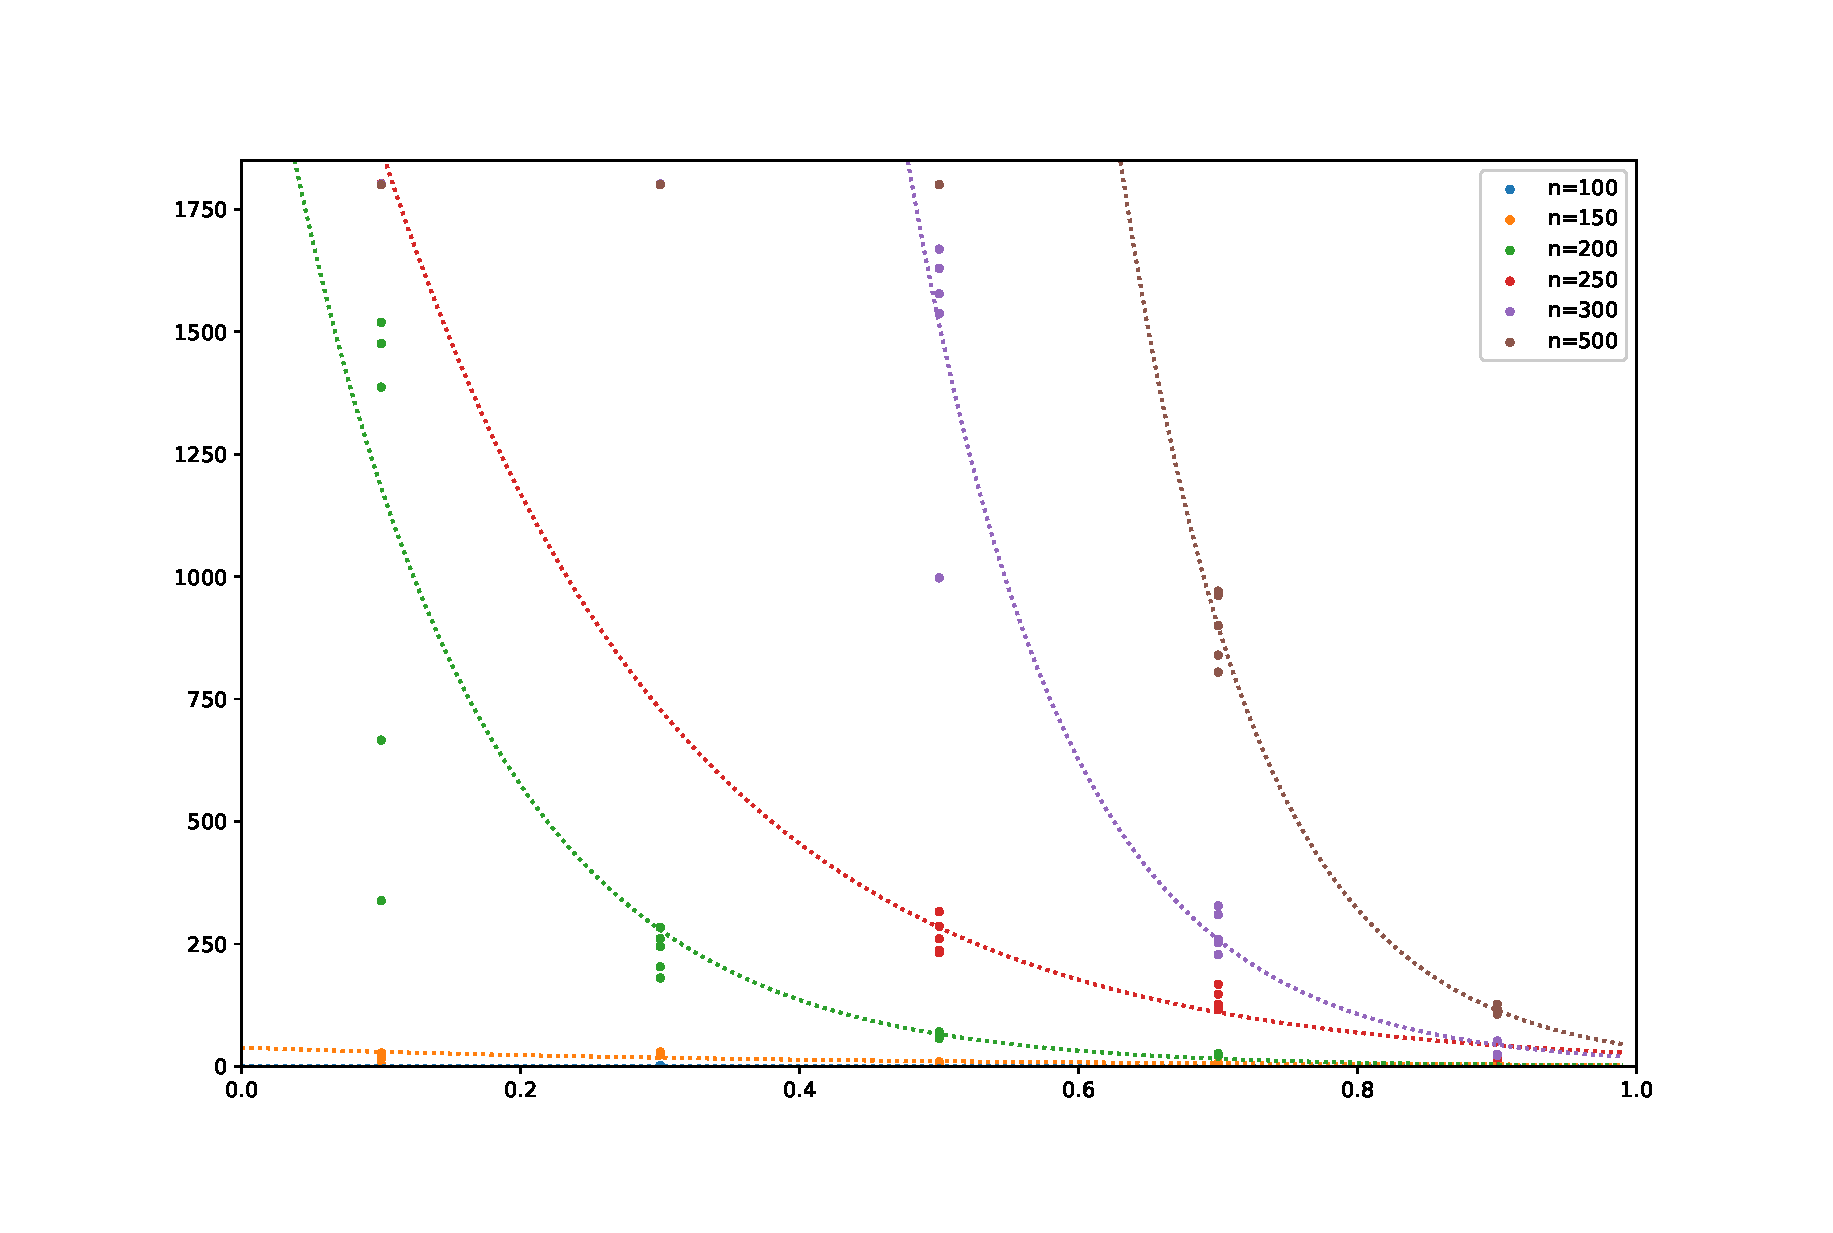
\includegraphics[scale=0.4]{images/gnp-2d.eps}
       \caption{Correlazione tra tempo di risoluzione $time$ (ordinata) e probabilità di generazione di ciascun arco $p$ (ascissa).}
        \label{fig:gnp2d}
\end{figure}

Oltre al semplice plot dei dati, in questo grafico è stata estrapolata una curva da ciascuno degli insiemi di misurazioni corrispondenti ad ogni dimensione (applicando la regressione lineare), in modo tale da riuscirne ad approssimare l'andamento. La regressione è naturalmente stata fatta esclusivamente per le misurazioni di $time$ inferiori al time limit. Il grafico risultante evidenzia una chiara relazione di tipo esponenziale inverso tra $p$ e $time$, per qualsiasi valore del parametro grandezza utilizzato. 

Anche la dimensione dell'istanza di grafo sembra giocare un ruolo relativamente importante nella determinazione della complessità del problema di vertex cover associato, essendo apparentemente responsabile per la velocità con cui l'esponenziale satura.
Per approfondire meglio il ruolo della dimensione nella determinazione della complessità di risoluzione si è rappresentato graficamente l'andamento del tempo di risoluzione al variare della dimensione del grafo e a parità di valori del parametro $p$. I risultati ottenuti sono riportati in Figura \ref{fig:gnpp}.

\begin{figure}[h!]
     \centering
       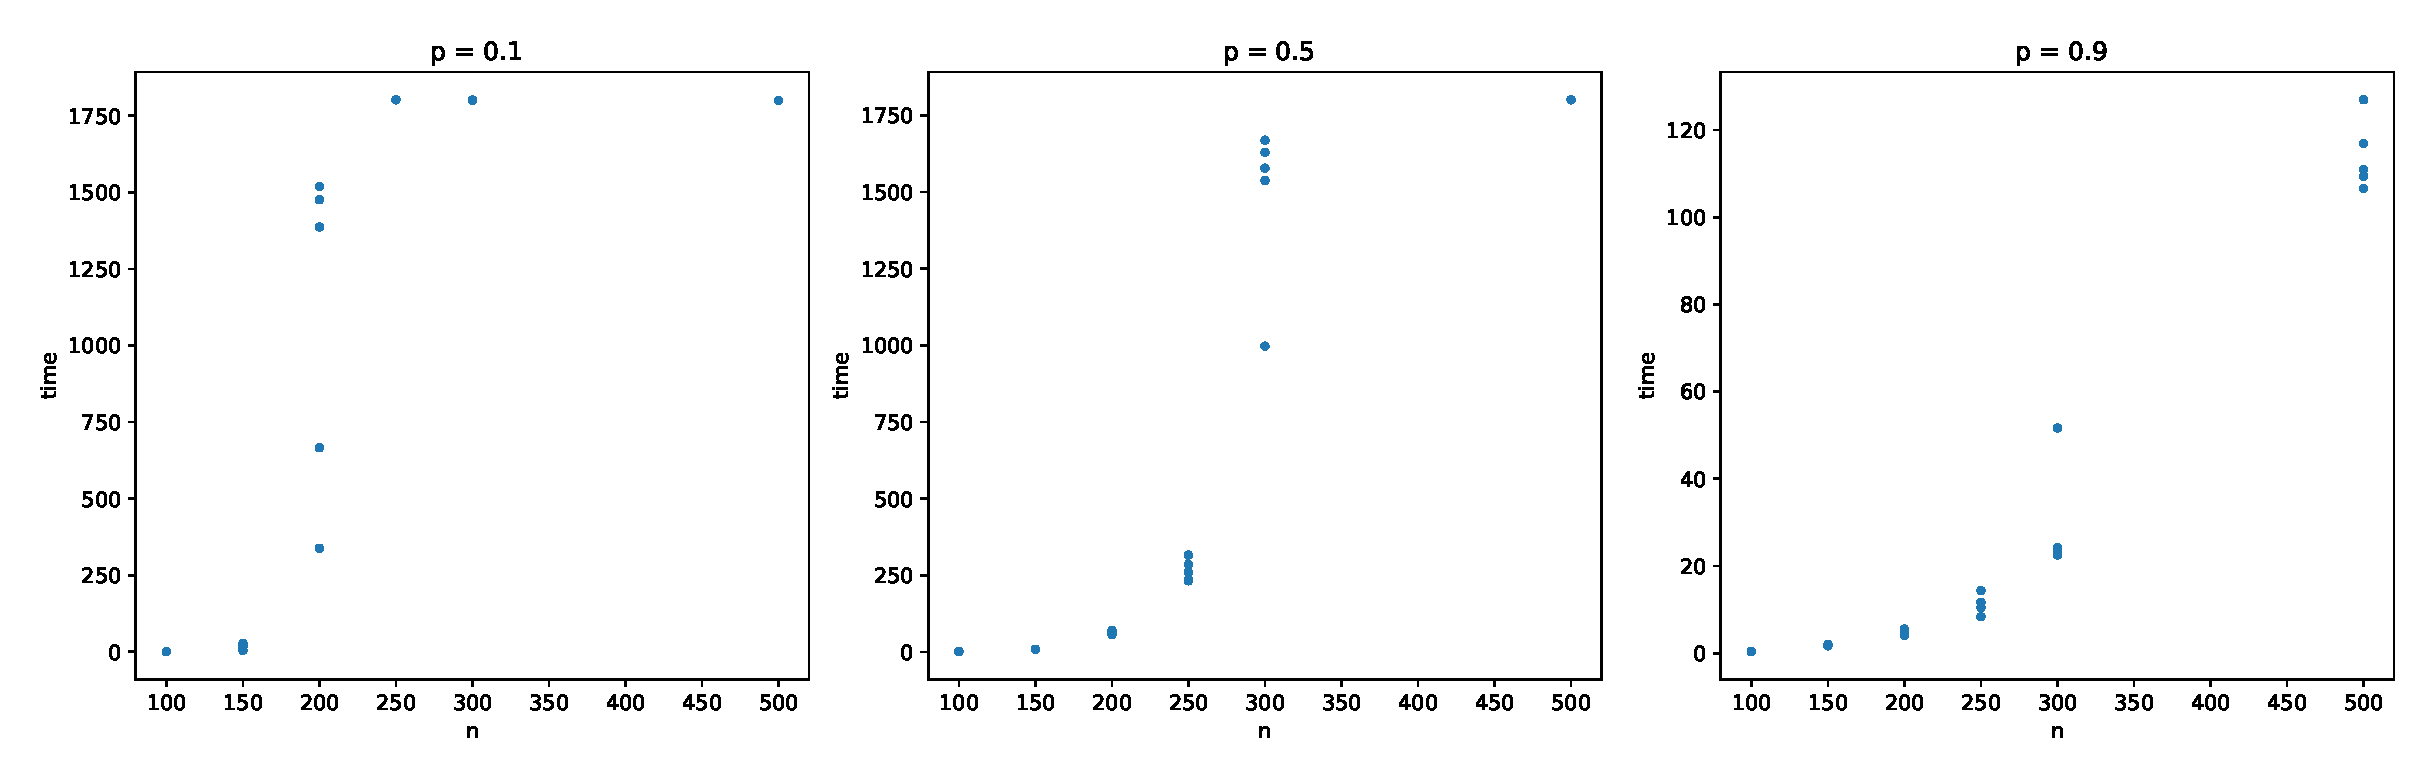
\includegraphics[scale=0.4]{images/gnp_p.eps}
       \caption{Correlazione tra tempo di risoluzione $time$ (ordinata) e dimensione del grafo $n$ (ascissa) per diversi valori di probabilità fissata $p=0.1$, $p=0.5$ e $p=0.9$.}
        \label{fig:gnpp}
\end{figure}

Come si può evincere dal grafo precedente, istanze di grafi più grandi diventano computazionalmente intrattabili molto prima rispetto a istanze dalla dimensione più contenuta, a parità di $p$. Tuttavia, come dimostra il grafico in Figura \ref{fig:gnpp} ottenuto per $p=0.9$,  il contributo dato dal numero di nodi alla complessità di risoluzione sembra essere secondario rispetto al ruolo giocato invece da $p$. 

In Figura \ref{fig:gnp3d} viene infine riportato un grafico tridimensionale riassuntivo, che rappresenta in un'unica immagine il variare della complessità del problema rispetto ad entrambi i parametri utilizzati nella generazione del grafo.
\vspace{-0cm}
\begin{figure}[h!]
     \centering
       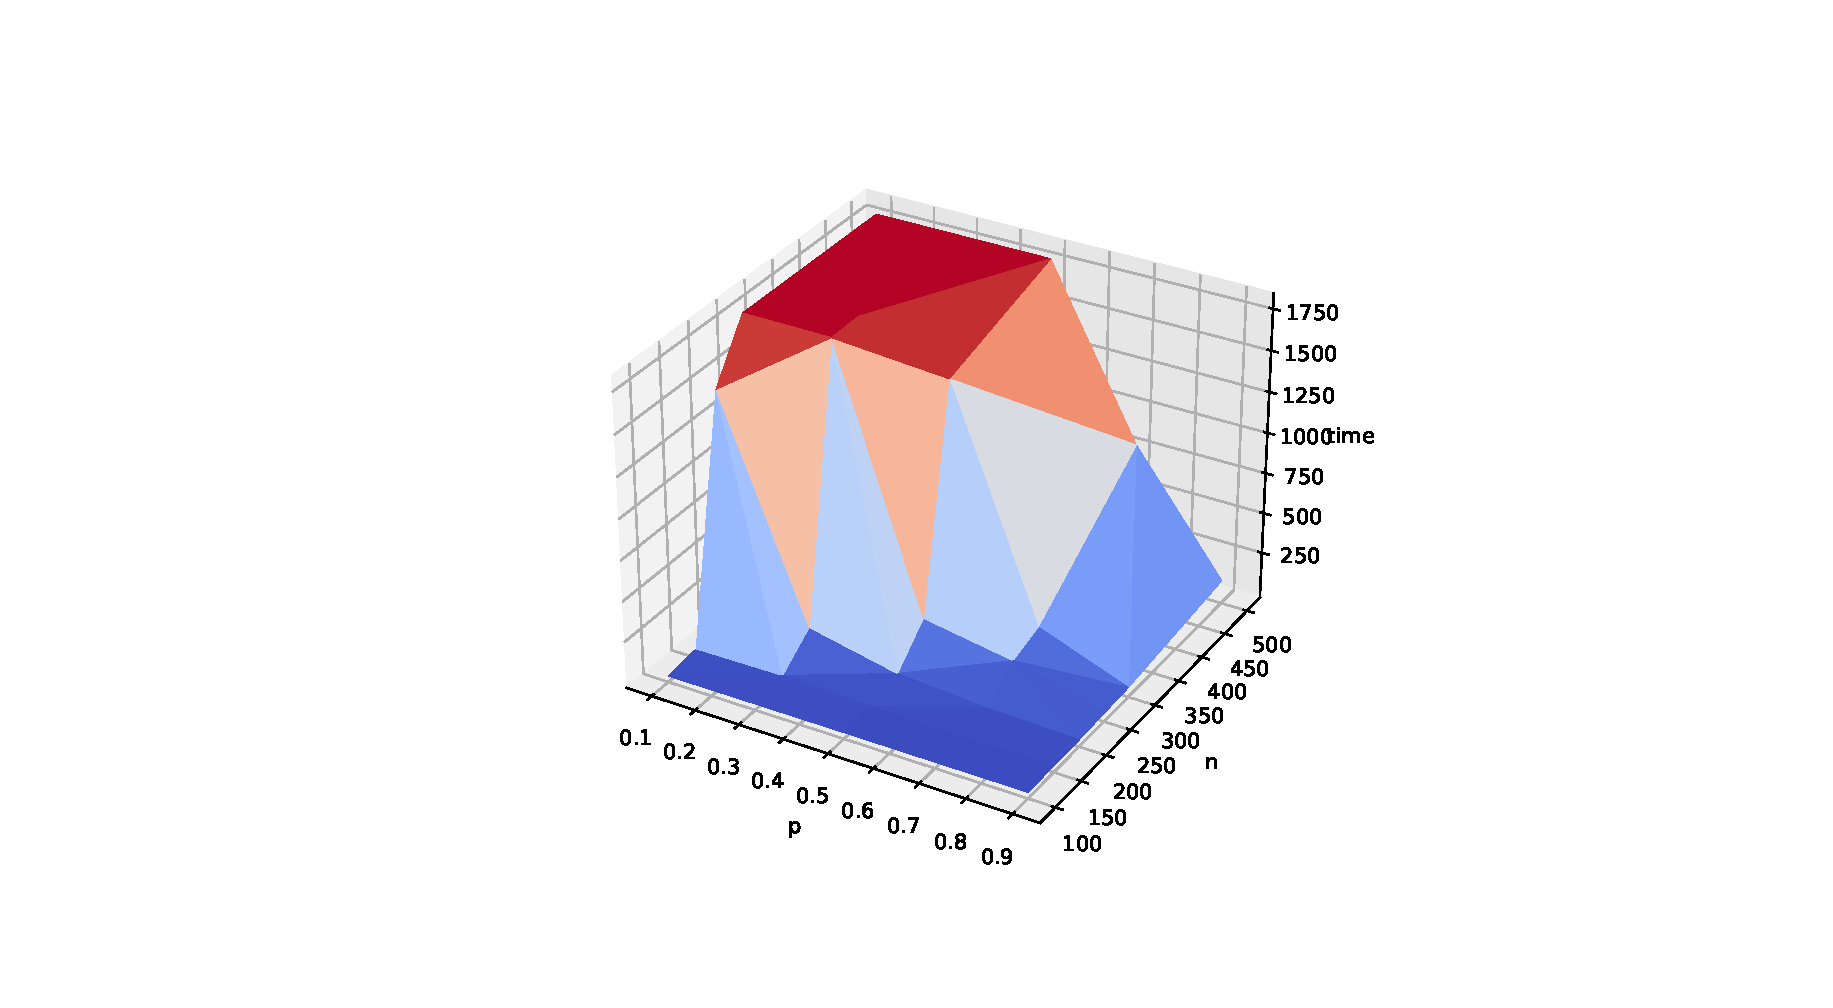
\includegraphics[scale=0.5]{images/gnp-3d.eps}
       \caption{Andamento della complessità del problema di vertex cover per grafi $G(n,p)$ al variare dei parametri $p$ ed $n$.}
        \label{fig:gnp3d}
\end{figure}

\section{Grafi regolari}

\section{Grafi di Watts-Strogatz}

\section{Grafi di Barabási-Albert}